\chapter{Annexe}

\chapter{Fichier créer pour HERBS}

\section{Les protéines associé à un organisme}

Ce qui suit sont deux extraits de fichier \texttt{csv} avec le point-virgule comme séparateur, des données représente les protéines prédites  dans différents organismes.
Ces protéines proviennent de différentes ressources et donc qu'une même protéine  peut avoir un identifiant différent, c'est la raison pour laquelle une étiquette unique est attribué. Les colonnes utilisées sont:
\begin{itemize}
	\item la colonne 1 pour l'étiquette
	\item la colonne 5 pour l'identifiant de l'organisme
	\item la colonne 6 pour l'identifiant de la réaction MetaCyc
\end{itemize}
 
 Deux autres colonnes pouvant avoir de l'intérêt, la colonne 10 pour l'identifiant \texttt{TrEMBL} et la colonne 11 qui est la référence finale d'\texttt{UniProt}.

\needspace{15\baselineskip}
\begin{adjustbox}{width=\textwidth}
\begin{lstlisting}[basicstyle=\tiny\normalfont\ttfamily,caption=LysineAAA.csv]
SSO0723;-3;616781;617791;14;1.1.1.87-RXN;117720;Q9UXB2;NULL;Q9UXB2;SULSO00653;DERAFNT;5985;;WANPAGS;4872
SSO0104;3;85752;86957;14;2-AMINOADIPATE-AMINOTRANSFERASE-RXN;113264;P95957;NULL;P95957;SULSO00092;RLNFTYV;48514;;QNVAFVP;56248
SSO2470;-1;2240677;2241174;14;HOMOACONITATE-HYDRATASE-RXN;116977;Q97VY3;NULL;Q97VY3;SULSO02199;YKAEPFP;310072;;QINTDDI;358441
SSO2471;-1;2241175;2242425;14;HOMOACONITATE-HYDRATASE-RXN;116976;Q97VY2;NULL;Q97VY2;SULSO02200;VIPFDHQ;295760;;LPDHYIF;358392
SSO0977;1;835585;836970;14;HOMOCITRATE-SYNTHASE-RXN;114153;Q97ZE0;NULL;Q97ZE0;SULSO00885;YTTSVAR;58663;;RDYVIDK;69000
SSO2470;-1;2240677;2241174;14;RXN3O-1983;116977;Q97VY3;NULL;Q97VY3;SULSO02199;YKAEPFP;310072;;QINTDDI;358441
SSO2471;-1;2241175;2242425;14;RXN3O-1983;116976;Q97VY2;NULL;Q97VY2;SULSO02200;VIPFDHQ;295760;;LPDHYIF;358392
SSO0159;3;132570;133430;14;RXN-5181;113282;Q7SI95;NULL;Q7SI95;SULSO00137;EFGYPCV;107728;;VFYVQEF;125752
SSO0156;3;131130;131924;14;RXN-5182;113279;Q980X0;NULL;Q980X0;SULSO00134;VGRFTDE;98613;;FMTKKVM;124653
SSO0155;2;130070;131128;14;RXN-5183;113278;Q980X1;NULL;Q980X1;SULSO00133;VCRIAVH;293480;;VRGSNFC;347614
SSO0160;2;133415;134593;14;RXN-5184;113283;Q7SI94;NULL;Q7SI94;SULSO00138;EPDIFTA;5485;;VFEPGEH;16661
SSO0162;3;134541;135581;14;RXN-5185;113284;Q980W5;NULL;Q980W5;SULSO00139;GDSDLDH;298917;;GDSDLDH;75994
PF0940;3;904320;905387;121;1.1.1.87-RXN;540962;NULL;Q8U299;Q8U299;PYRFU00928;MMPDDWR;5979;;TEDFYVG;4855
PF0121;-2;126676;127917;121;2-AMINOADIPATE-AMINOTRANSFERASE-RXN;542596;NULL;Q8U4G7;Q8U4G7;PYRFU00119;RLNFTYV;48514;;QNVAFVP;56248
PF1679;1;1561855;1562997;121;HOMOACONITATE-HYDRATASE-RXN;541348;Q8U0C0;NULL;Q8U0C0;PYRFU01667;AYIFFDH;295789;;RILLANM;358467
PF1680;3;1562994;1563488;121;HOMOACONITATE-HYDRATASE-RXN;541349;Q8U0B9;NULL;Q8U0B9;PYRFU01668;ITPGRYN;310086;;ITPGRYN;358450
\end{lstlisting}
\end{adjustbox}
	
\needspace{15\baselineskip}
\begin{adjustbox}{width=\textwidth}
\begin{lstlisting}[basicstyle=\tiny\normalfont\ttfamily,caption=LysineDAP.csv]
SSO0160;2;133415;134593;14;SUCCINYLDIAMINOPIMTRANS-RXN;113283;SSO0160;Q7SI94;NULL;0;Q7SI94;SULSO00138;5485;EPDIFTA;;;16661;VFEPGEH
SSO0876;-2;746826;748166;14;ASPARTATEKIN-RXN;117636;SSO0876;NULL;Q97ZL7;0;Q97ZL7;SULSO00796;293533;RIPRLSY;;;347652;HHINIAM
SSO1538;-1;1390102;1391334;14;SUCCDIAMINOPIMDESUCC-RXN;117368;SSO1538;NULL;Q97Y12;0;Q97Y12;SULSO01375;298928;ESETHKS;;;79093;DEECGGA
MTH52;1;31459;32691;15;RXN-7737;111885;MTH52;O26158;NULL;0;O26158;METTH00050;68338;KCAIEFR;;;80191;KCAIEFR
MTH272;2;208448;209065;15;2.3.1.89-RXN;111995;MTH272;NULL;O26372;0;O26372;METTH00268;271735;TRIWHHA;;;252544;NILVREQ
MTH802;-3;730683;731903;15;ASPARTATEKIN-RXN;111465;MTH802;NULL;O26893;0;O26893;METTH00792;293539;GSEVIHH;;;347665;AFLLGHC
MTH1334;-3;1200942;1201811;15;DIAMINOPIMEPIM-RXN;111174;MTH1334;O27389;NULL;0;O27389;METTH01300;317759;VPHAVIF;;;362430;CFARFVL
MTH1335;-1;1201817;1203103;15;DIAMINOPIMDECARB-RXN;111173;MTH1335;O27390;NULL;0;O27390;METTH01301;303690;HPKISTG;;;354153;NKFGIPI
MTH799;-3;727905;728948;15;ASPARTATE-SEMIALDEHYDE-DEHYDROGENASE-RXN;111468;199extraCds;O26890;NULL;199extraCds;O26890;METTH00789;293481;VIDGHTE;;;347615;ASCHRVP
MTH800;-3;728961;729782;15;DIHYDROPICRED-RXN;111467;199extraCds;O26891;NULL;199extraCds;O26891;METTH00790;303008;IVMAPNM;;;353543;IVMAPNM
MTH801;-2;729835;730686;15;DIHYDRODIPICSYN-RXN;111466;199extraCds;O26892;NULL;199extraCds;O26892;METTH00791;293604;ADAILCV;;;99624;HQKLFVE
MJ0571;3;508398;509819;16;ASPARTATEKIN-RXN;113860;MJ0571;Q57991;NULL;0;Q57991;METJA00586;293521;SVDMIIQ;;;347647;GANIKMI
MJ0721;3;655122;656318;16;SUCCINYLDIAMINOPIMTRANS-RXN;114007;MJ0721;Q58131;NULL;0;Q58131;METJA00739;5476;GGTGCQP;;;16652;GHCHPHL
MJ1097;-1;1037197;1038513;16;DIAMINOPIMDECARB-RXN;115261;MJ1097;Q58497;NULL;0;Q58497;METJA01124;303690;HPKISTG;;;354153;NKFGIPI
MJ1119;1;1059445;1060332;16;DIAMINOPIMEPIM-RXN;114328;MJ1119;Q58519;NULL;0;Q58519;METJA01145;317759;VPHAVIF;;;362430;CFARFVL
MJ1391;-1;1338520;1339776;16;RXN-7737;115009;MJ1391;Q58786;NULL;0;Q58786;METJA01429;67862;YLRLAAC;;;79608;GIQMAGA
\end{lstlisting}
\end{adjustbox}

\section{Intégration des prédictions de protéines dans la base de faits CLIPS}
\needspace{50\baselineskip}
\begin{lstlisting}[style=python-style,caption=getProteinFacts.py]
#!/usr/bin/env python
import MySQLdb
from sys import argv
from os.path import realpath

def writer( fileDescriptor, splittedLine ):
    fileDescriptor.write( "(uniprot (id " + splittedLine[5]
                                          + ") (alias " + splittedLine[0]
                                          + " sp:" + splittedLine[12]  + "))\n" )


def getOrganismNameBySid( db, Sid ):
    cursor = db.cursor()
    cursor.execute("SELECT O_id, O_species_code,"
                + " GROUP_CONCAT(REPLACE(REPLACE(REPLACE(name_txt,' ','_'),'(', '_'), ')', '_')"
                + " ORDER BY level SEPARATOR ' ') AS Lineage FROM Organism O INNER JOIN O_Taxonomy"
                + " USING(O_id) INNER JOIN Replicon USING(O_id) INNER JOIN Sequence USING(R_id) "
                + " WHERE S_id = %s GROUP BY O.O_id", [Sid])
    db.commit()
    numrows = int(cursor.rowcount)
    if numrows == 0:
        raise Exception("Id " + Sid + " not found in given database!" )
    return cursor.fetchone()

if __name__ == "__main__":

    if len( argv ) != 4:
        raise Exception( "Two parameters are expected. "
        					+ argv[0]
        					+ " <input> <processDataDir> <speciesDir>" )

    pkgdb = MySQLdb.connect(
                                host    = "mysqlagcdb.genoscope.cns.fr",
                                user    = "agc", 
                                passwd  = "xxxx", # secret :-)
                                db      = "pkgdb_dev"
                            )

    currentOrganismId   = None
    processFile         = None

    with open( argv[1], 'r' ) as input:
        for line in input:
            if not line.startswith( "Label" ):
                splittedLine = line.split(';')
                if splittedLine[4] != currentOrganismId:
                    if processFile != None: processFile.close() 
                    currentOrganismId   = splittedLine[4]
                    OId,species,lineage = getOrganismNameBySid( pkgdb, currentOrganismId )
                    processFile         = open( realpath( argv[2] + '/' + species + ".data"), "a+" )
                    speciesFile         = open( realpath( argv[3] + '/' + species + ".data"), "a+" )
                    speciesFile.write( "(species lineage " + lineage + ")\n" )
                writer( processFile, splittedLine ) 

        if processFile != None: processFile.close()
\end{lstlisting}

\needspace{15\baselineskip}
\begin{lstlisting}[style=python-style,caption=mappingUER\_Metacyc.py]
#!/usr/bin/env python
from sys import argv

if __name__ == "__main__":
    if len( argv ) != 3:
        raise Exception( "Two parameters are expected. " + argv[0] +  " <input> <output>" )
    
    with open( argv[1], 'r' ) as input:
        with open( argv[2], 'a+' ) as output:
            for line in input:
                start = line.find( "UER" )
                if start != -1:
                    fields= line[start:].split( )
                    output.write( "(observer uniprot define " + fields[0] + " -> and " + fields[2] + ")\n" )
\end{lstlisting}

\section{Fichier de correspondance protéines et réaction enzymatique d'UniPathway (UER)}

Ces fichiers de correspondances sont tabulés pour décrire les colonnes: description, id UER, id RHEA, id MetaCyc, variant métabolique.

\begin{adjustbox}{width=\textwidth}
\begin{lstlisting}[basicstyle=\tiny\normalfont\ttfamily,tabsize=2,showtabs=true,caption=AAA\_uer\_metacyc.tsv]
alpha-aminoadipate from 2-oxoglutarate: step 1/5	UER00028	RHEA:12929	HOMOCITRATE-SYNTHASE-RXN	LYSINE-AMINOAD-PWY : lysine biosynthesis IV 
PWY-3081 : lysine biosynthesis V 
P241-PWY : coenzyme B biosynthesis 
L-alpha-aminoadipate from 2-oxoglutarate: step 1/5	UER00028	-	HOMOCITRATE-SYNTHASE-RXN	LYSINE-AMINOAD-PWY : lysine biosynthesis IV 
PWY-3081 : lysine biosynthesis V 
P241-PWY : coenzyme B biosynthesis 
L-alpha-aminoadipate from 2-oxoglutarate: step 2/5	UER00029	RHEA:26101	RXN3O-1983	LYSINE-AMINOAD-PWY : lysine biosynthesis IV 
PWY-3081 : lysine biosynthesis V 
P241-PWY : coenzyme B biosynthesis 
L-alpha-aminoadipate from 2-oxoglutarate: step 2/5	UER00029	-	RXN3O-1983	LYSINE-AMINOAD-PWY : lysine biosynthesis IV 
PWY-3081 : lysine biosynthesis V 
P241-PWY : coenzyme B biosynthesis 
L-alpha-aminoadipate from 2-oxoglutarate: step 3/5	UER01027	RHEA:15485	HOMOACONITATE-HYDRATASE-RXN	LYSINE-AMINOAD-PWY : lysine biosynthesis IV 
PWY-3081 : lysine biosynthesis V 
P241-PWY : coenzyme B biosynthesis 
L-alpha-aminoadipate from 2-oxoglutarate: step 3/5	UER01027	-	RXN3O-1983	LYSINE-AMINOAD-PWY : lysine biosynthesis IV 
PWY-3081 : lysine biosynthesis V 
P241-PWY : coenzyme B biosynthesis 
L-alpha-aminoadipate from 2-oxoglutarate: step 4/5	UER00030	RHEA:11900	RXN-7970	PWY-3081 : lysine biosynthesis V 
LYSINE-AMINOAD-PWY : lysine biosynthesis IV 
P241-PWY : coenzyme B biosynthesis 
L-alpha-aminoadipate from 2-oxoglutarate: step 4/5	UER00030	-	RXN-7970	PWY-3081 : lysine biosynthesis V 
LYSINE-AMINOAD-PWY : lysine biosynthesis IV 
P241-PWY : coenzyme B biosynthesis 
L-alpha-aminoadipate from 2-oxoglutarate: step 5/5	UER00031	RHEA:12601	2-AMINOADIPATE-AMINOTRANSFERASE-RXN	LYSINE-AMINOAD-PWY : lysine biosynthesis IV 
PWY-3081 : lysine biosynthesis V 
LYSINE-DEG1-PWY : lysine degradation II 
PWY-5283 : lysine degradation V 
L-alpha-aminoadipate from 2-oxoglutarate: step 5/5	UER00031	-	2-AMINOADIPATE-AMINOTRANSFERASE-RXN	LYSINE-AMINOAD-PWY : lysine biosynthesis IV 
PWY-3081 : lysine biosynthesis V 
LYSINE-DEG1-PWY : lysine degradation II 
PWY-5283 : lysine degradation V 
L-lysine from L-alpha-aminoadipate (Thermus route): step 1/5	UER00035	-	RXN-5181	PWY-3081 : lysine biosynthesis V 
L-lysine from L-alpha-aminoadipate (Thermus route): step 2/5	UER00036	-	RXN-5182	PWY-3081 : lysine biosynthesis V 
L-lysine from L-alpha-aminoadipate (Thermus route): step 3/5	UER00037	RHEA:28590	RXN-5183	PWY-3081 : lysine biosynthesis V 
L-lysine from L-alpha-aminoadipate (Thermus route): step 3/5	UER00037	-	RXN-5183	PWY-3081 : lysine biosynthesis V 
L-lysine from L-alpha-aminoadipate (Thermus route): step 4/5	UER00038	RHEA:28594	RXN-5184	PWY-3081 : lysine biosynthesis V 
L-lysine from L-alpha-aminoadipate (Thermus route): step 4/5	UER00038	-	RXN-5184	PWY-3081 : lysine biosynthesis V 
L-lysine from L-alpha-aminoadipate (Thermus route): step 5/5	UER00039	RHEA:28598	RXN-5185	PWY-3081 : lysine biosynthesis V 
L-lysine from L-alpha-aminoadipate (Thermus route): step 5/5	UER00039	-	RXN-5185	PWY-3081 : lysine biosynthesis V 
L-lysine from L-alpha-aminoadipate (fungal route): step 1/3	UER00032	-	RXN-10855	LYSINE-AMINOAD-PWY : lysine biosynthesis IV 
L-lysine from L-alpha-aminoadipate (fungal route): step 1/3	UER00032	-	RXN-8173	LYSINE-AMINOAD-PWY : lysine biosynthesis IV 
PWY-5283 : lysine degradation V 
LYSINE-DEG1-PWY : lysine degradation II 
PWY-5298 : lysine degradation VI 
PWY-5314 : lysine degradation VIII 
PWY-5324 : lysine degradation IX 
L-lysine from L-alpha-aminoadipate (fungal route): step 2/3	UER00033	RHEA:10020	RXN3O-127	LYSINE-AMINOAD-PWY : lysine biosynthesis IV 
L-lysine from L-alpha-aminoadipate (fungal route): step 2/3	UER00033	-	RXN3O-127	LYSINE-AMINOAD-PWY : lysine biosynthesis IV 
L-lysine from L-alpha-aminoadipate (fungal route): step 3/3	UER00034	RHEA:12440	1.5.1.7-RXN	LYSINE-AMINOAD-PWY : lysine biosynthesis IV 
L-lysine from L-alpha-aminoadipate (fungal route): step 3/3	UER00034	-	1.5.1.7-RXN	LYSINE-AMINOAD-PWY : lysine biosynthesis IV 
\end{lstlisting}
\end{adjustbox}

\begin{adjustbox}{width=\textwidth}
\begin{lstlisting}[basicstyle=\tiny\normalfont\ttfamily,tabsize=2,showtabs=true,caption=DAP\_uer\_metacyc.tsv]
(S)-tetrahydrodipicolinate from L-aspartate: step 1/4	UER00015	RHEA:23776	ASPARTATEKIN-RXN	DAPLYSINESYN-PWY : lysine biosynthesis I 
PWY-2941 : lysine biosynthesis II 
PWY-2942 : lysine biosynthesis III 
PWY-5097 : lysine biosynthesis VI 
HOMOSERSYN-PWY : homoserine biosynthesis 
PWY-6562 : norspermidine biosynthesis 
P101-PWY : ectoine biosynthesis 
PWY-6559 : spermidine biosynthesis II 
PWY-7153 : grixazone biosynthesis 
(S)-tetrahydrodipicolinate from L-aspartate: step 2/4	UER00016	RHEA:24284	ASPARTATE-SEMIALDEHYDE-DEHYDROGENASE-RXN	DAPLYSINESYN-PWY : lysine biosynthesis I 
PWY-2941 : lysine biosynthesis II 
PWY-2942 : lysine biosynthesis III 
PWY-5097 : lysine biosynthesis VI 
HOMOSERSYN-PWY : homoserine biosynthesis 
PWY-6562 : norspermidine biosynthesis 
P101-PWY : ectoine biosynthesis 
PWY-6559 : spermidine biosynthesis II 
PWY-7153 : grixazone biosynthesis 
(S)-tetrahydrodipicolinate from L-aspartate: step 3/4	UER00017	RHEA:34171	DIHYDRODIPICSYN-RXN	DAPLYSINESYN-PWY : lysine biosynthesis I 
PWY-2941 : lysine biosynthesis II 
PWY-2942 : lysine biosynthesis III 
PWY-5097 : lysine biosynthesis VI 
(S)-tetrahydrodipicolinate from L-aspartate: step 3/4	UER00017	-	DIHYDRODIPICSYN-RXN	DAPLYSINESYN-PWY : lysine biosynthesis I 
PWY-2941 : lysine biosynthesis II 
PWY-2942 : lysine biosynthesis III 
PWY-5097 : lysine biosynthesis VI 
(S)-tetrahydrodipicolinate from L-aspartate: step 4/4	UER00018	RHEA:35331	RXN-14014	DAPLYSINESYN-PWY : lysine biosynthesis I 
PWY-2942 : lysine biosynthesis III 
PWY-2941 : lysine biosynthesis II 
PWY-5097 : lysine biosynthesis VI 
(S)-tetrahydrodipicolinate from L-aspartate: step 4/4	UER00018	-	RXN-14014	DAPLYSINESYN-PWY : lysine biosynthesis I 
PWY-2942 : lysine biosynthesis III 
PWY-2941 : lysine biosynthesis II 
PWY-5097 : lysine biosynthesis VI 
DL-2,6-diaminopimelate from (S)-tetrahydrodipicolinate: step 1/1	UER00026	RHEA:13561	DIAMINOPIMELATE-DEHYDROGENASE-RXN	PWY-2942 : lysine biosynthesis III 
DL-2,6-diaminopimelate from (S)-tetrahydrodipicolinate: step 1/1	UER00026	RHEA:24797	RXN-4821	PWY-2942 : lysine biosynthesis III 
DL-2,6-diaminopimelate from LL-2,6-diaminopimelate: step 1/1	UER00025	RHEA:15393	DIAMINOPIMEPIM-RXN	DAPLYSINESYN-PWY : lysine biosynthesis I 
PWY-2941 : lysine biosynthesis II 
PWY-5097 : lysine biosynthesis VI 
L-lysine from DL-2,6-diaminopimelate: step 1/1	UER00027	RHEA:15101	DIAMINOPIMDECARB-RXN	DAPLYSINESYN-PWY : lysine biosynthesis I 
PWY-2941 : lysine biosynthesis II 
PWY-2942 : lysine biosynthesis III 
PWY-5097 : lysine biosynthesis VI 
LL-2,6-diaminopimelate from (S)-tetrahydrodipicolinate (acetylase route): step 1/3	UER00022	RHEA:13085	2.3.1.89-RXN	PWY-2941 : lysine biosynthesis II 
LL-2,6-diaminopimelate from (S)-tetrahydrodipicolinate (acetylase route): step 2/3	UER00023	RHEA:25315	RXN-4822	PWY-2941 : lysine biosynthesis II 
LL-2,6-diaminopimelate from (S)-tetrahydrodipicolinate (acetylase route): step 3/3	UER00024	RHEA:20405	N-ACETYLDIAMINOPIMELATE-DEACETYLASE-RXN	PWY-2941 : lysine biosynthesis II 
LL-2,6-diaminopimelate from (S)-tetrahydrodipicolinate (aminotransferase route): step 1/1	UER00466	RHEA:23988	RXN-7737	PWY-5097 : lysine biosynthesis VI 
LL-2,6-diaminopimelate from (S)-tetrahydrodipicolinate (succinylase route): step 1/3	UER00019	RHEA:17325	TETHYDPICSUCC-RXN	DAPLYSINESYN-PWY : lysine biosynthesis I 
LL-2,6-diaminopimelate from (S)-tetrahydrodipicolinate (succinylase route): step 2/3	UER00020	RHEA:11960	SUCCINYLDIAMINOPIMTRANS-RXN	DAPLYSINESYN-PWY : lysine biosynthesis I 
LL-2,6-diaminopimelate from (S)-tetrahydrodipicolinate (succinylase route): step 3/3	UER00021	RHEA:22608	SUCCDIAMINOPIMDESUCC-RXN	DAPLYSINESYN-PWY : lysine biosynthesis I 
\end{lstlisting}
\end{adjustbox}

\section{Les variants métabolique pour la biosynthèse de la lysine}
\begin{lstlisting}[basicstyle=\tiny\normalfont\ttfamily,caption=data/processes/lysine\_DAP\_biosynthesis.data]
;;;; -------------------------------------------------------
;;; HERBS (Hamap Expert Rules Based System)
;;;
;;; @file: lysine_AAA_biosynthesis.data
;;; -------------------------------------------------------
;;;
(process declare lysine_AAA_biosynthesis present in ALL)
(process define lysine_AAA_biosynthesis -> and UPA00033)
(process define UPA00033 -> or UPA00033-alt-0 UPA00033-alt-1)
(process define UPA00033-alt-0 -> and ULS00012 ULS00013)
(process define UPA00033-alt-1 -> and ULS00012 ULS00014)
(process define ULS00012 -> and ULS00012-alt-0)
(process define ULS00012-alt-0 -> and UER00028 UER00029 UER00030 UER00031 UER01027)
(process define ULS00013 -> or ULS00013-alt-0 ULS00013-alt-1)
(process define ULS00013-alt-0 -> and UER00032 UER00034)
(process define ULS00013-alt-1 -> and UER00033 UER00034)
(process define ULS00012 -> and ULS00012-alt-0)
(process define ULS00012-alt-0 -> and UER00028 UER00029 UER00030 UER00031 UER01027)
(process define ULS00014 -> or ULS00014-alt-0 ULS00014-alt-1)
(process define ULS00014-alt-0 -> and UER00035 UER00037 UER00038 UER00039)
(process define ULS00014-alt-1 -> and UER00036 UER00037 UER00038 UER00039)
\end{lstlisting}

\begin{lstlisting}[basicstyle=\tiny\normalfont\ttfamily,caption=data/processes/lysine\_DAP\_biosynthesis.data]
;;;; -------------------------------------------------------
;;; HERBS (Hamap Expert Rules Based System)
;;;
;;; @file: lysine_DAP_biosynthesis.data
;;; -------------------------------------------------------
;;;
(process declare lysine_DAP_biosynthesis present in ALL)
(process define lysine_DAP_biosynthesis -> and UPA00034)
(process define UPA00034 -> or UPA00034-alt-0 UPA00034-alt-1 UPA00034-alt-2 )
(process define UPA00034-alt-0  -> and ULS00006 ULS00007 ULS00009 ULS00010 ULS00011)
(process define UPA00034-alt-1  -> and ULS00006 ULS00008 ULS00009 ULS00010 ULS00011)
(process define UPA00034-alt-2  -> and ULS00006 ULS00227 ULS00009 ULS00010 ULS00011)
(process define ULS00006 -> or ULS00006-alt-0 ULS00006-alt-1 )
(process define ULS00006-alt-0  -> and UER00015 UER00016 UER00017)
(process define ULS00006-alt-1  -> and UER00015 UER00018 UER00017)
(process define ULS00007 -> and ULS00007-alt-0 )
(process define ULS00007-alt-0  -> and UER00019 UER00020 UER00021)
(process define ULS00009 -> and ULS00009-alt-0 )
(process define ULS00009-alt-0  -> and UER00025)
(process define ULS00010 -> and ULS00010-alt-0 )
(process define ULS00010-alt-0  -> and UER00026)
(process define ULS00011 -> and ULS00011-alt-0 )
(process define ULS00011-alt-0  -> and UER00027)
(process define ULS00006 -> or ULS00006-alt-0 ULS00006-alt-1 )
(process define ULS00006-alt-0  -> and UER00015 UER00016 UER00017)
(process define ULS00006-alt-1  -> and UER00015 UER00018 UER00017)
(process define ULS00008 -> and ULS00008-alt-0 )
(process define ULS00008-alt-0  -> and UER00022 UER00023 UER00024)
(process define ULS00009 -> and ULS00009-alt-0 )
(process define ULS00009-alt-0  -> and UER00025)
(process define ULS00010 -> and ULS00010-alt-0 )
(process define ULS00010-alt-0  -> and UER00026)
(process define ULS00011 -> and ULS00011-alt-0 )
(process define ULS00011-alt-0  -> and UER00027)
(process define ULS00006 -> or ULS00006-alt-0 ULS00006-alt-1 )
(process define ULS00006-alt-0  -> and UER00015 UER00016 UER00017)
(process define ULS00006-alt-1  -> and UER00015 UER00018 UER00017)
(process define ULS00227 -> and ULS00227-alt-0 )
(process define ULS00227-alt-0  -> and UER00466)
(process define ULS00009 -> and ULS00009-alt-0 )
(process define ULS00009-alt-0  -> and UER00025)
(process define ULS00010 -> and ULS00010-alt-0 )
(process define ULS00010-alt-0  -> and UER00026)
(process define ULS00011 -> and ULS00011-alt-0 )
(process define ULS00011-alt-0  -> and UER00027)
\end{lstlisting}


\chapter{Schéma des différentes notions abordé par GROOLS}

\begin{shadedfigure}
	\centering
	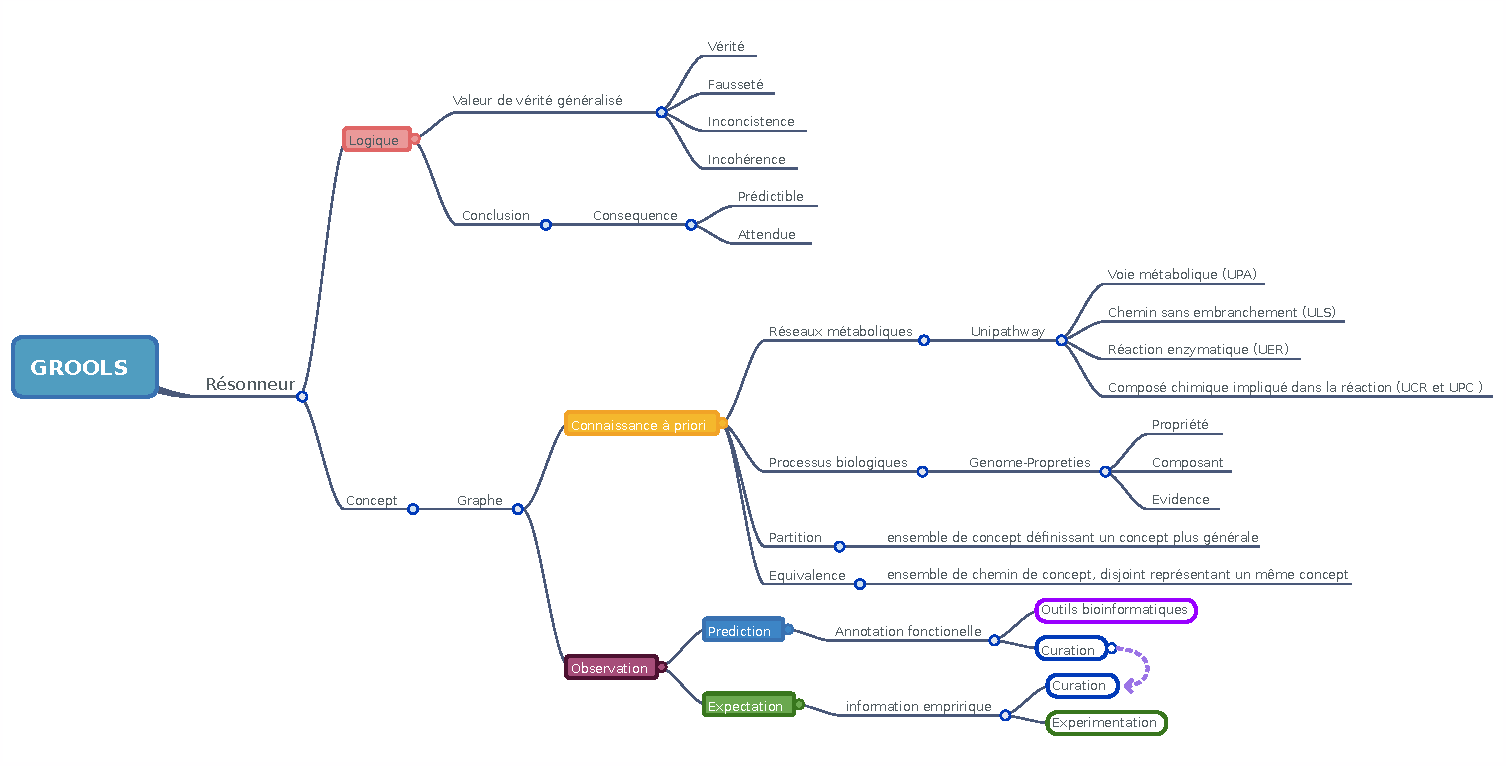
\includegraphics[width=\textwidth]{img/GROOLS_mindmap.pdf}
	\caption{  }
	\label{fig:GROOLS_mindmap}
\end{shadedfigure}
